\newpage
\section{Benutzungsoberfläche}
\subsection{Allgemeiner Aufbau}
In den Abbildungen \ref{ui-max} und \ref{ui-min} wird der  Entwurf des Hauptnutzerinterface gezeigt. Generell betrachtet ist die Oberfläche in zwei Bereiche geteilt. Im oberen Abschnitt befindet sich der Kopfbereich. Dieser stimmt in allen für den Endnutzer bestimmten Anwendungsbereichen überein. Darunter liegt eine Sektion, die den einzelnen Unterbereichen der Seite zur Verfügung steht.

\subsection{Ziffernerkennung}
Dieser Teil der Anwendung ist die Hauptansicht und ist vorrangig für den Endanwender gedacht. Sie dient hauptsächlich der Eingabe einer Ziffer und deren Erkennung. Außerdem wird eine Suchfunktion nach vorhandenen Netzen, ein Infobereich mit Eigenschaften des Netzes und Konsole zur Ausgabe von Berechnungsinformationen zur Verfügung gestellt. Der rechte  Bereich mit den zusätzlichen Informationen kann ausgeblendet werden. Dadurch steht für andere Bereiche der Anwendung mehr Platz zur Verfügung. Insbesondere bei kleineren Anzeigegeräten wie Tablets oder anderen mobilen Geräten kommt dieser Fakt zum Tragen. In Abbildung \ref{ui-max} ist die maximierte und in der darauffolgenden(\ref{ui-min}) ist die minimierte Variante zu sehen.
 
 \paragraph{Elemente der Ziffernerkennungs-Oberfläche}
 \begin{enumerate}
 	\item Anwendungskopf
 	\item Sprachauswahl
 	\item Suchfeld mit Bestätigungsschaltfläche
 	\item Liste der Suchergebnisse
 	\item Feld zum Zeichnen einer Ziffer
 	\item Feld zur Anzeige des Ergebnisses
 	\item Konsole mit Berechnungsinformationen
 	\item Bereich zur Darstellung zusätzlicher Informationen zum geladenen Netz
 \end{enumerate}
 
\begin{figure}[H]
 
 	\centering
 	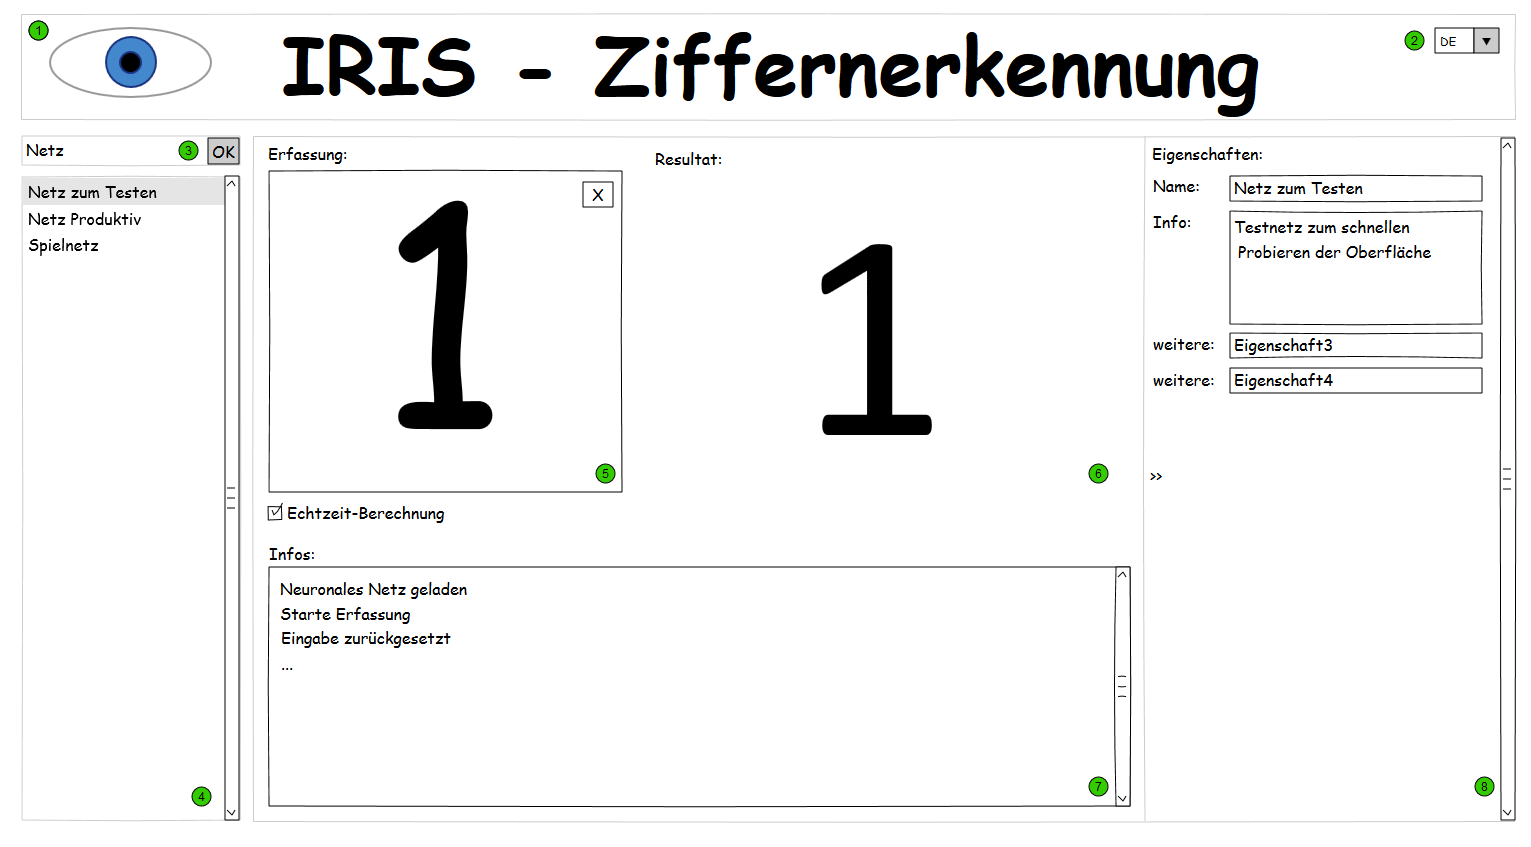
\includegraphics[height=0.75\textwidth, angle=90]{Abbildungen/UI-Mocks/Main-Ui.png}
 	\caption{Nutzeroberfläche mit eingeblendeten Metainformationen}
 	\label{ui-max}
\end{figure}

\begin{figure}[H]
	\centering
	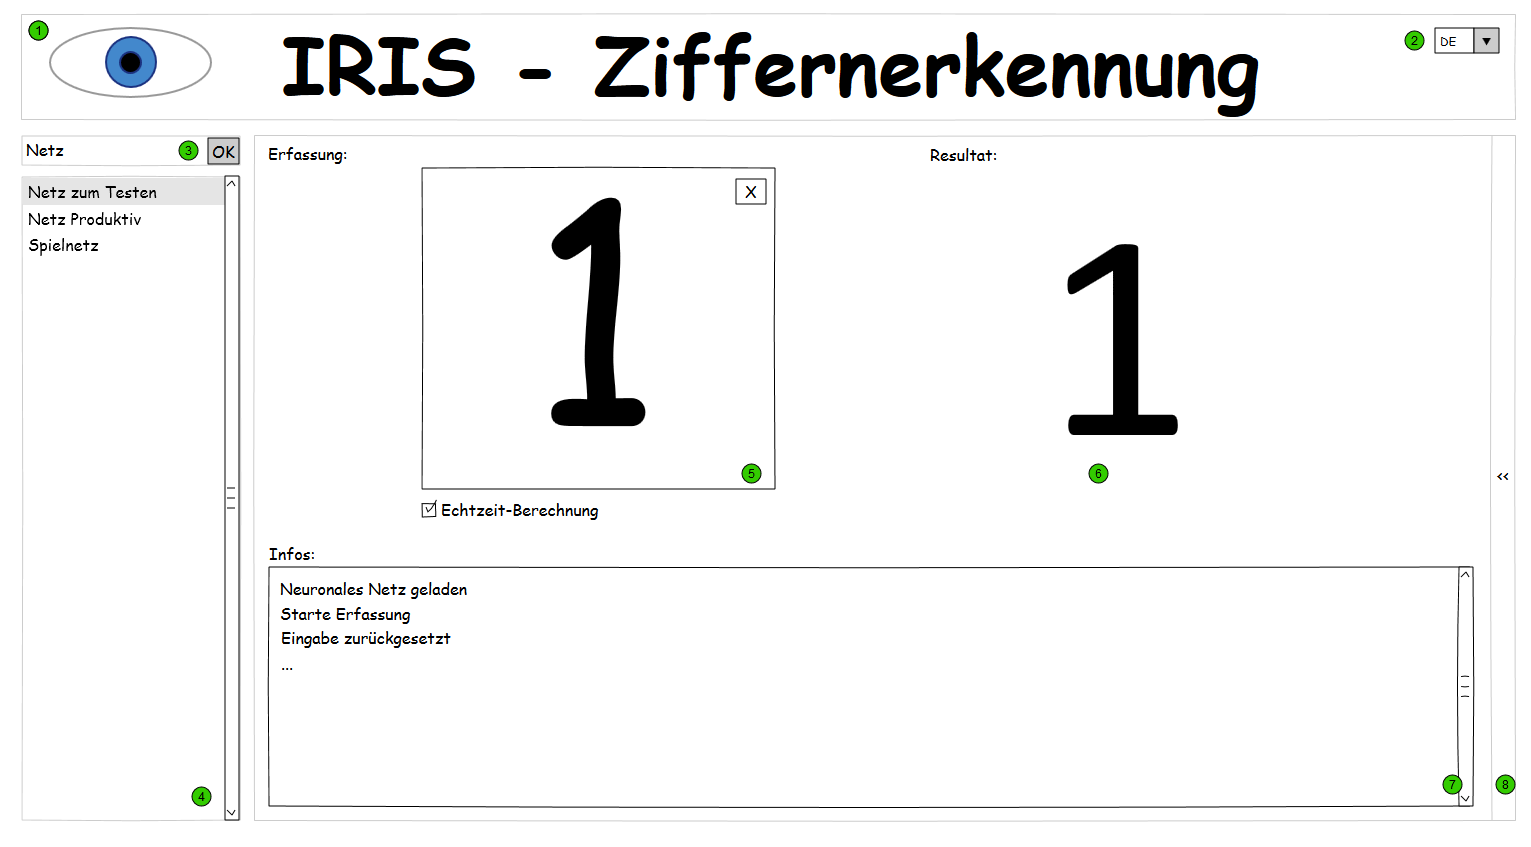
\includegraphics[height=0.75\textwidth, angle=90]{Abbildungen/UI-Mocks/Main-Ui-Minimized.png}
	\caption{Nutzeroberfläche mit ausgeblendeten Metainformationen}
	\label{ui-min}
\end{figure}

\subsection{Datenzugriff auf neuronale Netze}
Dieser Abschnitt ist für Administratoren und Entwickler entworfen. Über sie können neuronale Netze erstellt, verändert und wieder gespeichert werden. Die Grundaufteilung ist analog zur Ziffernerkennungsoberfläche und stellt auch eine Sprachauswahl und Suche bereit. Für die Zukunft, ist die Möglichkeit vorgesehen, Netze über Schaltflächen und Regler für die Eigenschaften dieser zu erstellen. In der ersten Realisierung wird aber nur die Eingabe von JSON zur Bestimmung der Struktur des Netzes implementiert. Separat zu erwähnen ist die Möglichkeit zum schnellen Wechsel von der  Datenbearbeitungs- zur Trainingsseite. Abbildung \ref{ui-crud} zeigt den Entwurf der Datenzugriffsseite.

 \paragraph{Elemente der Datenzugriffs-Oberfläche} (zur Erkennungsansicht(\ref{ui-max}) abweichende)
 \begin{enumerate}
 	\item Manipulation der zusätzlichen Netzinformationen
 	\item Sektion zur Netzstruktur
 	\item Auswahl der Eingabeart
 	\item Textfeld für die Eingabe über JSON
 	\item Neuanlegen eines Datensatzes
 	\item Wechsel zum Training des geladenen Netzes
 	\item Verwerfen der aktuellen Änderungen
 	\item Speichern der eingegeben Daten
 \end{enumerate}

\begin{figure}[H]
	\centering
	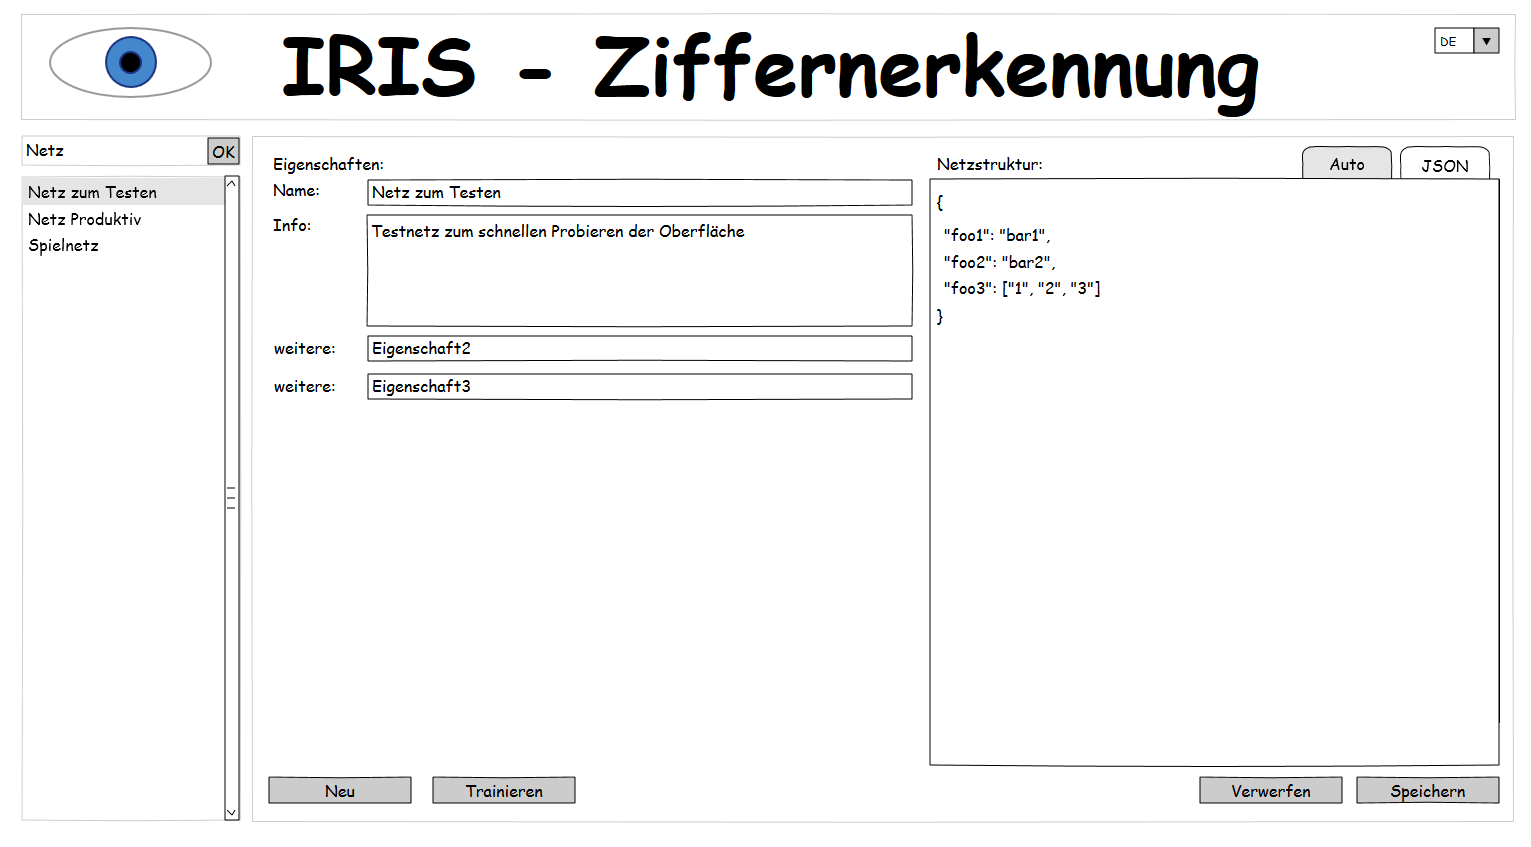
\includegraphics[width=1\textwidth]{Abbildungen/UI-Mocks/CRUD-Ui.png}
	\caption{Nutzeroberfläche zum Datenzugriff auf neuronale Netze}
	\label{ui-crud}
\end{figure}

\subsection{Training eines neuronale Netzes}
In diesem, für Entwickler und Administratoren gedachten Bereich, wird die Möglichkeit zum Trainings eines Netzes zur Verfügung gestellt. In Abbildung \ref{ui-train} wird der Aufbau dieses Anwendungsbereich dargestellt. Die grundlegende Struktur bleibt gleich und analog zur Datenmanipulationsseite wird ein schneller Wechsel zu dieser bereit gestellt. Hauptfunktion ist die Eingabe von Trainingsparametern und das Starten sowie Beenden eines Trainings. Je nach Erfolg kann das Resultat gespeichert oder verworfen werden.

\paragraph{Elemente der Trainings-Oberfläche} (zur Erkennungsansicht(\ref{ui-max}) abweichende)
\begin{enumerate}
\item Eingabe der Trainingsparameter
\item Ausgabe von Berechnungsinformationen und Lernerfolg
\item Wechsel zur Bearbeitung des geladenen Netzes
\item Starten des Trainings
\item Stoppen des Trainings
\item Verwerfen der Resultate
\item Speichern der Resultate
\end{enumerate}

\begin{figure}[H]
	\centering
	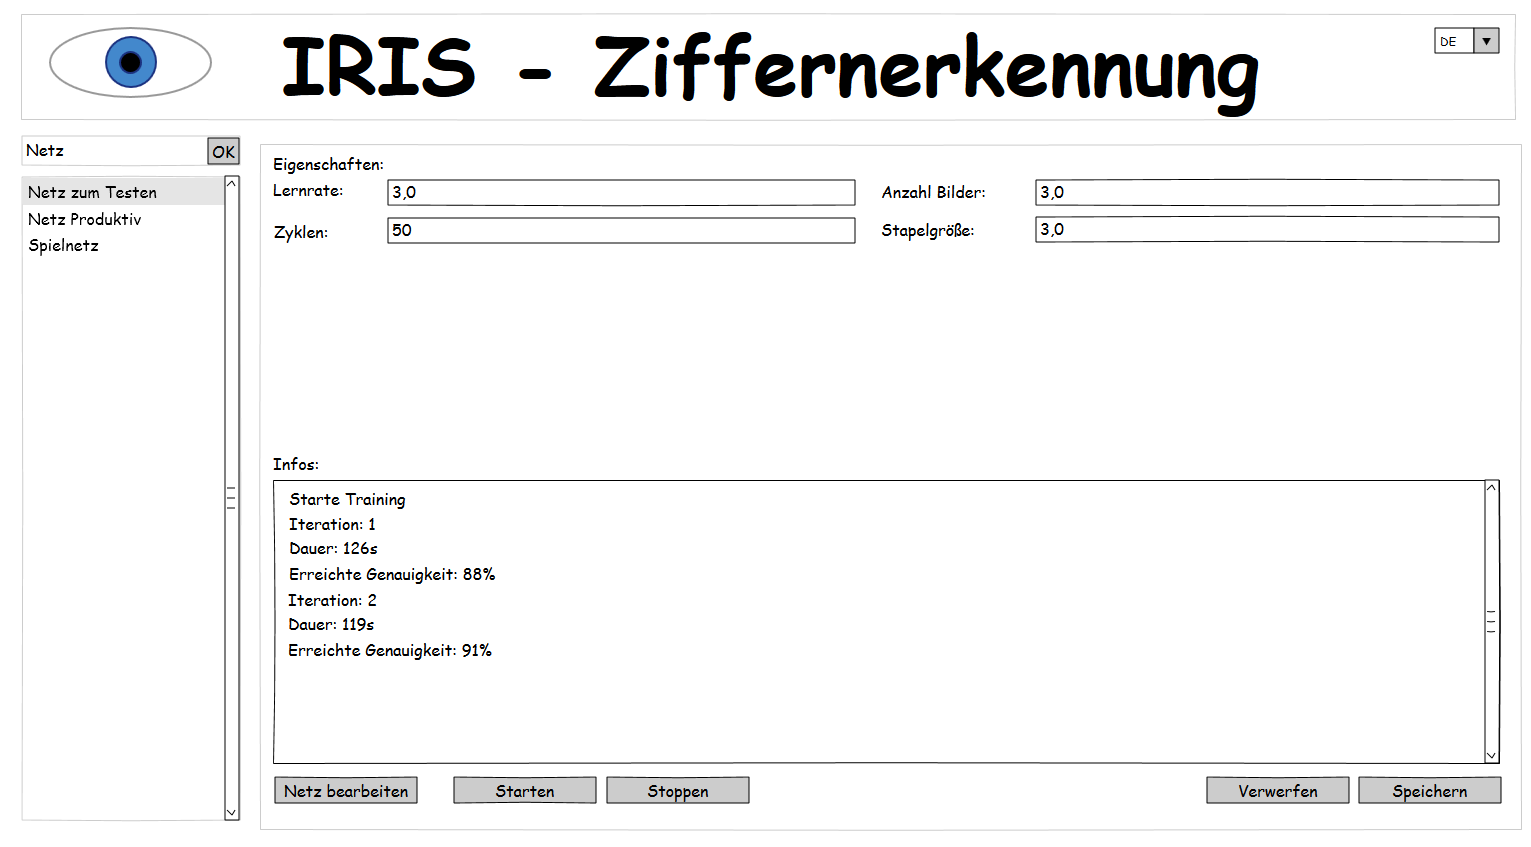
\includegraphics[width=1\textwidth]{Abbildungen/UI-Mocks/Train-Ui.png}
	\caption{Nutzeroberfläche zum Training eines Netzes}
	\label{ui-train}
\end{figure}
